\documentclass[titlepage,landscape]{seminar}
\usepackage{url}
\usepackage{graphicx}
\usepackage{hyperref}
\usepackage{epstopdf}
\usepackage{slides}

\newcommand{\frack}{\frac{1}{k}}

\begin{document}

\myslide{
\heading{Statiscal vs. evolutionary sampling}

\begin{itemize}

\item {\it Statistical sampling} - Repeated samples from the same
  population differ from one another. For example, the sample
  frequency of an allele, $\hat p$, will differ from sample to sample
  even if the ``true'' population frequency, $p$, is always the same. 

\item {\it Genetic (or evolutionary) sampling} - We are rarely, if
  ever, interested only in the populations or loci we sampled. We are
  almost always interested in using them as ``representatives'' of all
  populations or loci that could have been sampled. In other words the
  populations and loci we actually studied are best regarded as a
  sample from the set of all comparable populations and loci that
  could have been studied.

\end{itemize}
}

\myslide{
\heading{Statiscal vs. evolutionary sampling}
\begin{center}
\includegraphics[height=0.9\textheight]{sampling.eps}
\end{center}
\vfill\eject
}

\myslide{
\heading{$F$-statistics: a Bayesian approach}

The data
\begin{eqnarray*}
n_{11,i} &=& \hbox{\# of $A_1A_1$ genotypes} \\
n_{12,i} &=& \hbox{\# of $A_1A_2$ genotypes} \\
n_{22,i} &=& \hbox{\# of $A_2A_2$ genotypes} \\
i         &=& \hbox{population index} \\
I         &=& \hbox{number of populations} \\
\end{eqnarray*}

\vfill\eject

}

\myslide{
\heading{$F$-statistics: a Bayesian approach}

The data
\begin{eqnarray*}
n_{11,i} &=& \hbox{\# of $A_1A_1$ genotypes} \\
n_{12,i} &=& \hbox{\# of $A_1A_2$ genotypes} \\
n_{22,i} &=& \hbox{\# of $A_2A_2$ genotypes} \\
i         &=& \hbox{population index} \\
I         &=& \hbox{number of populations} \\
\end{eqnarray*}

The genotype frequencies
\begin{eqnarray*}
x_{11,i} &=& p_{i}^2 + fp_{i}(1-p_{i}) \\
x_{12,i} &=& 2p_{i}(1-p_{i})(1-f) \\
x_{22,i} &=& (1-p_{i})^2 + fp_{i}(1-p_{i})
\end{eqnarray*}

\vfill\eject

}

\myslide{
\heading{$F$-statistics: a Bayesian approach}

The likelihood
\[
P({\bf n}|{\bf p},f) \propto \prod_{i=1}^I x_{11,i}^{n_{11,i}}
x_{12,i}^{n_{12,i}} x_{22,i}^{n_{22,i}}
\]

\vfill\eject
  
}

\myslide{
\heading{$F$-statistics: a Bayesian approach}

The likelihood
\[
P({\bf n}|{\bf p},f) \propto \prod_{i=1}^I x_{11,i}^{n_{11,i}}
x_{12,i}^{n_{12,i}} x_{22,i}^{n_{22,i}}
\]

The distribution of allele frequencies among populations
\[
P({\bf p}|{\bf\bar p}, \theta)
\]

\vfill\eject
  
}

\myslide{
\heading{$F$-statistics: a Bayesian approach}
\begin{center}
\includegraphics[height=0.9\textheight]{sampling.eps}
\end{center}
\vfill\eject
}

\myslide{
\heading{$F$-statistics: a Bayesian approach}

The likelihood
\[
P({\bf n}|{\bf p},f) \propto \prod_{i=1}^I x_{11,i}^{n_{11,i}}
x_{12,i}^{n_{12,i}} x_{22,i}^{n_{22,i}}
\]

The distribution of allele frequencies among populations
\[
P({\bf p}|{\bf\bar p}, \theta)
\]

The posterior distribution of $\theta$ and $f$
\[
P(f,\theta|{\bf\bar p},\theta,f) \propto
P({\bf n}|{\bf p},f) P({\bf p}|{\bf\bar p},\theta) P({\bf\bar p})P(\theta)P(f)
\]

\vfill\eject
  
}

\myslide{
\heading{$F$-statistics: extending the Bayesian approach}

So far we've assumed that every locus shows the same amount of
differentiation and that every population is equally divergent from
every other.

\begin{eqnarray*}
  \theta_i &=& \mbox{locus-specific $\theta$} \\
  \theta_k &=& \mbox{population-specific $\theta$} \\
  \theta_{ik} &=& \mbox{population- and locus-specific $\theta$}
\end{eqnarray*}

Algebra gets more complicated, but implementing is straightforward.

\vfil\eject

}

\myslide{
\heading{$F_{ST}$ outliers}

\begin{center}
  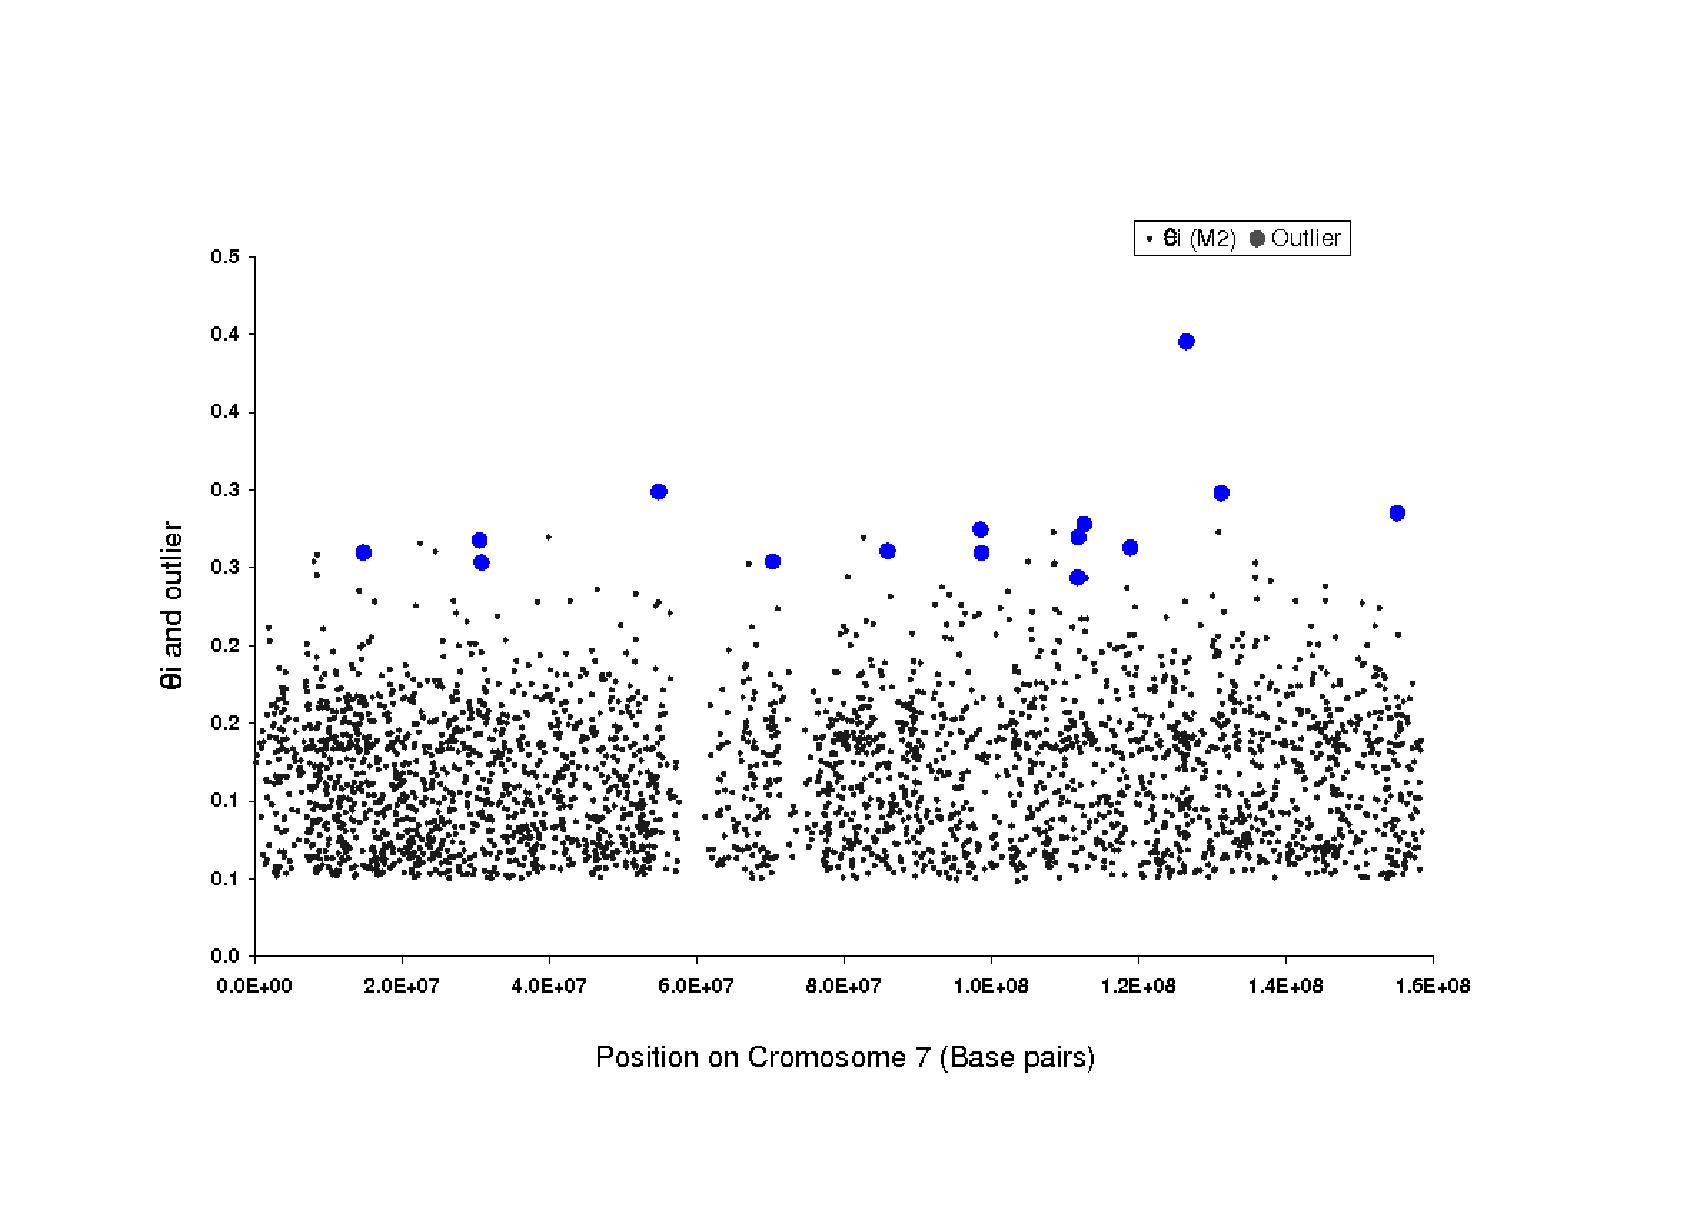
\includegraphics[height=7cm]{outlier.eps}
\end{center}

}

\myslide{
\heading{$F$-statistics: an important limitation}

$F$-statistics are great, \emphasis{but using them requires us to
  specify which individuals belong to which populations before we
  start the analysis}.

\emphasis{Question}: Is there a way to use the data we have to tell us what
populations individuals belong to?
}

\myslide{
\heading{Individual assignment using {\tt STRUCTURE}}
  
\begin{eqnarray*}
\mbox{P}(i|k) &=& \frac{\mbox{P}(x_i|\gamma_k)}{\sum_k
  \mbox{P}(x_i|\gamma_k)} \\
x_i &=& \mbox{genotype of individual $i$} \\
\gamma_k &=& \mbox{genotype frequencies in population $k$}
\end{eqnarray*}
For example, if $A_1A_1$ is labeled as $1$, $A_1A_2$ as $2$, $A_2A_2$
as 3, and we assume that genotypes are in Hardy-Weinberg, then
\begin{eqnarray*}
\mbox{P}((1,2,2,1,3)|(p_{k1}, p_{k2}, p_{k3}, p_{k4}, p_{k5})) = (p_{k1}^2)(2p_{k2}q_{k2})(2p_{k3}q_{k3})(p_{k4}^2)(q_{k5}^2)
\end{eqnarray*}
}

\myslide{
\heading{Using {\tt STRUCTURE} in barberry}
  
{\it Berberis thunbergii\/}
\begin{itemize}
\item 85 feral, 7 horticultural, 4 cultivated
\item 147 polymorphic AFLP markers
\end{itemize}
\begin{table}
\begin{center}
\begin{tabular}{cc}
\hline\hline
K & Mean L(K) \\
\hline
2 & -2553.2 \\
3 & {\bf -2331.9} \\
4 & -2402.9 \\
5 & -2476.3 \\
\hline
\end{tabular}
\end{center}
\caption{Mean log probability of the data for $K=2,3,4,5$ in the {\it
    Berberis thunbergii\/} data}
\end{table}
}

\myslide{
\heading{Using {\tt STRUCTURE} in barberry}

  \begin{figure}
\resizebox{\textwidth}{!}{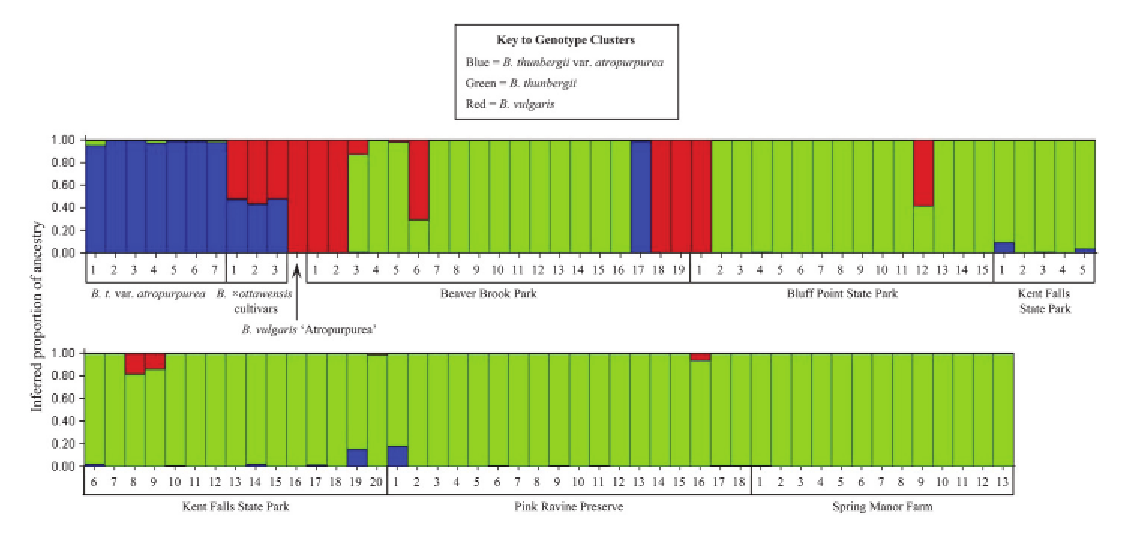
\includegraphics{lubell-structure.eps}}
\caption{Analysis of AFLP data from {\it Berberis
    thunbergii}}
\end{figure}
}

\myslide{
\heading{Using {\tt STRUCTURE} in humans}
  
\begin{itemize}

\item Human Genome Diversity Cell Line Panel (HGDP-CEPH)

\item 1056 individuals, 52 geographic populations, 377 autosomal
  microsatellite loci

\end{itemize}

\begin{figure}
\resizebox{\textwidth}{!}{\includegraphics{HGDP-CEPH.eps}}
\end{figure}

}

\myslide{
  \heading{Picking $K$ in a STRUCTURE analysis}

\includegraphics[width=0.9\textwidth]{LabWork3GraphK.png}  
}

\myslide{
\heading{Principal components analysis of genotypes}

Principal components analysis is a ``dimension reduction'' method, a
way of reducing a very large number of variables to a smaller, more
manageable number for interpretation and analysis.

\begin{center}
  \includegraphics[height=5cm]{pca-example.eps}
\end{center}

\vfill\eject
}

\myslide{
\heading{Principal components analysis of genotypes}

3129 Europeans, 500,568 SNP loci

\begin{figure}
\begin{center}
\resizebox{0.5\textwidth}{!}{\includegraphics{human-PCA.eps}}
\end{center}
\end{figure}

}

\end{document}

